\documentclass[12pt]{book}
\usepackage[utf8]{inputenc}
\usepackage{graphicx}
\usepackage{hyperref}
\usepackage{amsmath}
\usepackage{amsfonts}
\usepackage{amssymb}
\usepackage{listings}
\usepackage{placeins}
\usepackage{graphicx}
\lstset{basicstyle=\ttfamily,breaklines=true}
%%%%%%%%%%%%%%%%%%%%%%%%%%%%%%%%%%%%%%%%%%%%%%%%%%%%%%%%%%%%%%%%%%%%%%%%
%  chapters/capitulo10.tex
\begin{document}
	%%%%%%%%%%%%%%%%%%%%%%%%%%%%%%%%%%%%%%%%%%%%%%%%%%%%%%%%%%%%%%%%%%%%%%%%
	\chapter{Optimización de Clustering para Segmentación Socioeconómica}
	\label{chap:10}
	\textbf{Autor}: \large{Eddy Kennedy Mamani Hallas}
	\section{Objetivos y criterios de clustering}
	El objetivo principal del clustering es dividir un conjunto de datos en grupos o clústeres de manera que los elementos dentro de cada grupo sean similares entre sí y diferentes de los elementos de otros grupos. 
	
	Un criterio fundamental es minimizar la varianza intra-clúster, lo que significa que los datos dentro de un clúster deben estar lo más cerca posible entre sí. Las métricas como el índice de Silhouette y el índice de Davies-Bouldin ayudan a evaluar la calidad del clustering, proporcionando indicadores sobre la cohesión interna de los grupos y la separación entre ellos.
	
	\section{Métodos de clustering}
	\subsection{K-Means}
	El algoritmo \textbf{K-Means} es uno de los métodos más populares y simples para realizar clustering. Se basa en la partición de datos en $k$ clústeres, donde cada clúster está representado por un centroide. El objetivo del algoritmo es minimizar la suma de las distancias cuadradas entre los datos y el centroide del clúster al que pertenecen.
	
	A pesar de su eficiencia, \textbf{K-Means} presenta limitaciones, como la sensibilidad a outliers y la necesidad de predefinir el número de clústeres ($k$). Además, el algoritmo puede converger a mínimos locales dependiendo de la inicialización de los centroides.
	
	\textbf{Ejemplo Aplicado:}
	Supongamos que tenemos un conjunto de datos con la edad y los ingresos anuales de un grupo de personas. Queremos agruparlas en 2 clústeres: un clúster para personas con edades más jóvenes y bajos ingresos, y otro para personas mayores con ingresos más altos. Aplicamos \textbf{K-Means} para segmentar los datos.
	
	\textbf{Datos:}
	\[
	\begin{array}{|c|c|}
		\hline
		\textbf{Edad (años)} & \textbf{Ingresos Anuales (USD)} \\
		\hline
		25 & 25000 \\
		30 & 27000 \\
		35 & 50000 \\
		40 & 55000 \\
		45 & 60000 \\
		50 & 100000 \\
		55 & 120000 \\
		60 & 130000 \\
		\hline
	\end{array}
	\]
	
	El algoritmo comienza con la asignación aleatoria de dos centroides y asigna a cada persona al clúster más cercano, luego recalcula los centroides y repite el proceso hasta la convergencia. El resultado sería:
	\begin{itemize}
		\item \textbf{Clúster 1 (Jóvenes, bajos ingresos):} Personas con edades entre 25 y 40 años y bajos ingresos.
		\item \textbf{Clúster 2 (Mayores, altos ingresos):} Personas mayores de 40 años con ingresos más altos.
	\end{itemize}
	\subsubsection*{Código de referencia}
	\textbf{K-Means:} Este es el primer ejemplo donde queremos agrupar a las personas según su edad e ingresos anuales. \\
	\textbf{Código en Python:} \\ \url{https://colab.research.google.com/drive/152HFVZmpswx1L7QdVLTu0z
	rWdE62oHNP?usp=sharing}
	
	\subsection{Clustering espectral}
	Este método se basa en la teoría de grafos para identificar grupos en datos complejos. Utiliza la matriz de similitud de los datos para construir un grafo donde los nodos representan datos y las aristas representan similitudes. Posteriormente, se aplica descomposición en valores propios para identificar las particiones.
	
	El clustering espectral es especialmente útil para datos que no son linealmente separables, aunque su complejidad computacional puede ser un desafío en conjuntos de datos grandes.
	
	\textbf{Ejemplo Aplicado:}
	Supongamos que tenemos una red social donde queremos identificar grupos de personas que interactúan frecuentemente entre sí. Los datos incluyen las interacciones de las personas con los demás (por ejemplo, las veces que han comentado o dado “me gusta” en las publicaciones de otros).
	
	\textbf{Matriz de Similitud (donde cada fila es una persona y cada columna indica la similitud de interacción con otras personas):}
	\[
	\begin{array}{|c|c|c|c|}
		\hline
		\textbf{Persona} & \textbf{Persona A} & \textbf{Persona B} & \textbf{Persona C} \\
		\hline
		\textbf{Persona 1} & 1.0 & 0.8 & 0.2 \\
		\textbf{Persona 2} & 0.8 & 1.0 & 0.5 \\
		\textbf{Persona 3} & 0.2 & 0.5 & 1.0 \\
		\hline
	\end{array}
	\]
	La matriz de similitud indica que Persona 1 tiene una interacción alta con Persona A y una baja interacción con Persona C. Al aplicar clustering espectral, obtenemos que:
	\begin{itemize}
		\item Persona 1 y Persona 2 forman un grupo (alta interacción).
		\item Persona 3 está en un grupo separado debido a la baja interacción con los otros.
	\end{itemize}
	\subsubsection*{Código de referencia}
	\textbf{Clustering Espectral:} Este es el ejemplo de un grafo de interacciones sociales. \\
	\textbf{Código en Python:} \\ \url{https://colab.research.google.com
		/drive/152HFVZmpswx1L7QdVLTu0zr
		WdE62oHNP?usp=sharing}
	
	\subsection{Clustering jerárquico}
	El clustering jerárquico construye una estructura de árbol (dendrograma) para organizar los datos. Existen dos enfoques principales: 
	\begin{itemize}
		\item Aglomerativo (bottom-up): Cada dato comienza como un clúster independiente, y los clústeres se fusionan iterativamente hasta formar un único grupo.
		\item Divisivo (top-down): Comienza con un único clúster que contiene todos los datos y se divide recursivamente en clústeres más pequeños.
	\end{itemize}
	El clustering jerárquico permite explorar diferentes niveles de granularidad, pero puede ser computacionalmente costoso.
	
	\textbf{Ejemplo Aplicado:}
	Imaginemos que tenemos un conjunto de datos sobre las preferencias de compra de productos (por ejemplo, productos electrónicos, ropa, y alimentos) de un grupo de clientes. Queremos agruparlos en clústeres para crear campañas de marketing personalizadas.
	
	\textbf{Datos:}
	\[
	\begin{array}{|c|c|c|c|}
		\hline
		\textbf{Cliente} & \textbf{Electrónica} & \textbf{Ropa} & \textbf{Alimentos} \\
		\hline
		1 & 5 & 3 & 1 \\
		2 & 4 & 2 & 3 \\
		3 & 2 & 5 & 4 \\
		4 & 1 & 2 & 5 \\
		\hline
	\end{array}
	\]
	Aplicando el método aglomerativo, comenzamos con cada cliente como un clúster independiente. Luego, el algoritmo comienza a fusionar los clústeres más similares basados en sus preferencias de compra. El dendrograma podría indicar que los Clientes 1 y 2 tienen preferencias similares, por lo que se agrupan, y luego los Clientes 3 y 4 se agrupan en otro clúster, lo que da lugar a dos grupos:
	\begin{itemize}
		\item Clúster 1: Clientes interesados principalmente en productos electrónicos.
		\item Clúster 2: Clientes interesados en ropa y alimentos.
	\end{itemize}
	\subsubsection*{Código de referencia}
	\textbf{Clustering Jerárquico:} Este es el ejemplo de un dendrograma para mostrar cómo se agrupan los clientes. \\
	\textbf{Código en Python:} \\ \url{https://colab.research.google.com/drive/152HFVZmpswx1L7QdVLTu0zrWdE62oHNP?usp=sharing}
	
	\section{Optimización de asignaciones de clustering}
	
	\subsection{Mini-Batch K-Means}
	El algoritmo \textbf{Mini-Batch K-Means} es una extensión del algoritmo K-Means diseñada para manejar grandes volúmenes de datos. En lugar de usar todo el conjunto de datos en cada iteración, el algoritmo trabaja con pequeños subconjuntos aleatorios (mini-batches), lo que reduce significativamente el tiempo de cálculo.
	
	\textbf{Ejemplo aplicado:}
	Supongamos que tenemos datos de 1 millón de compras en línea. Usando \textbf{Mini-Batch K-Means}, el algoritmo toma pequeños lotes de 1,000 compras a la vez para agrupar a los clientes según su comportamiento de compra, acelerando el proceso.
	\subsubsection*{Código de referencia}
	\textbf{Mini-Batch K-Means:} Este es un ejemplo con un conjunto de datos más grande, usando Mini-Batch K-Means. \\
	\textbf{Código en Python:} \\ \url{https://colab.research.google.com/drive/152HFVZmpswx1L7QdVLTu0zrWdE62oHNP?usp=sharing}
	
	\subsection{Paralelización}
	La \textbf{paralelización} permite distribuir las tareas computacionales entre múltiples núcleos de procesamiento para mejorar la eficiencia cuando se manejan grandes volúmenes de datos.
	
	\textbf{Ejemplo aplicado:}
	Imaginemos que tenemos datos de tráfico web de millones de usuarios. Usando la librería \texttt{Joblib} en Python, podemos distribuir el proceso de clustering entre varios núcleos de procesamiento para acelerar el análisis.
	
	\begin{lstlisting}[language=Python]
		from joblib import Parallel, delayed
		import numpy as np
		
		# Simulación de un conjunto de datos
		X = np.random.rand(1000000, 10) 
		# 1 millón de registros
		
		# Función para ajustar el modelo de K-Means
		def fit_kmeans(X_batch):
		# Aquí se colocaría el código de K-Means
		pass
		
		# Paralelización del proceso
		results = Parallel(n_jobs=4)(delayed(fit_kmeans)
		(X[i:i+1000]) for i in range(0, len(X), 1000))
	\end{lstlisting}
	\subsubsection*{Código de referencia}
	\textbf{Paralelización:} Usamos Joblib para paralelizar el proceso de clustering. \\
	\textbf{Código en Python:} \\ \url{https://colab.research.google.com/drive/152HFVZmpswx1L7QdVLTu0zrWdE62oHNP?usp=sharing}
	
	\FloatBarrier
	\section{Análisis socioeconómico en Huancavelica}
	El análisis basado en el Censo Nacional 2017 reveló que Huancavelica es la región con mayor incidencia de pobreza en el Perú, afectando al 75.2\% de su población, como se muestra en la figura \ref{fig:peru_pobreza}.
	
	\begin{figure}[H]
		\centering
		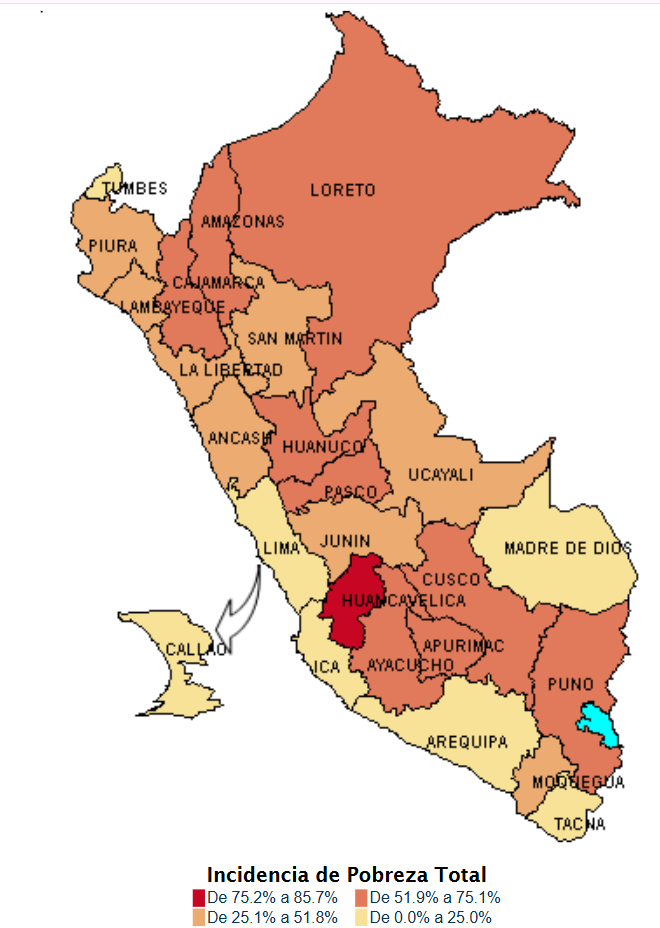
\includegraphics[width=0.5\textwidth]{peru_pobreza.png}
		\caption{Mapa de la incidencia de pobreza total en Perú (2017).}
		\label{fig:peru_pobreza}
	\end{figure}
	\FloatBarrier
	\section{Dataset utilizado}
	En esta sección, se presenta una tabla descriptiva con los datos de viviendas en los distritos de Huancavelica, detallando las viviendas ocupadas, desocupadas y abandonadas, según el Censo Nacional 2007.
	
	\begin{table}[H]
		\centering
		\resizebox{\textwidth}{!}{%
			\begin{tabular}{|l|r|r|r|r|}
				\hline
				\textbf{Distrito} & \textbf{Viviendas Ocupadas} & \textbf{Viviendas Desocupadas} & \textbf{Viviendas Abandonadas} \\
				\hline
				Huancavelica       & 140024  & 16795 & 13464 \\
				Acobamba            & 11000   & 1000  & 700   \\
				Angaraes            & 13500   & 1500  & 1000  \\
				Castrovirreyna      & 9500    & 500   & 300   \\
				Churcampa           & 10500   & 500   & 350   \\
				Huaytará            & 8500    & 500   & 250   \\
				Tayacaja            & 16500   & 1500  & 1000  \\
				\hline
			\end{tabular}%
		}
		\caption{Datos de viviendas en los distritos de Huancavelica.}
		\label{tab:huancavelica_viviendas}
	\end{table}
	
	A continuación, se presenta una imagen del dataset utilizado:
	
	\begin{figure}[H]
		\centering
		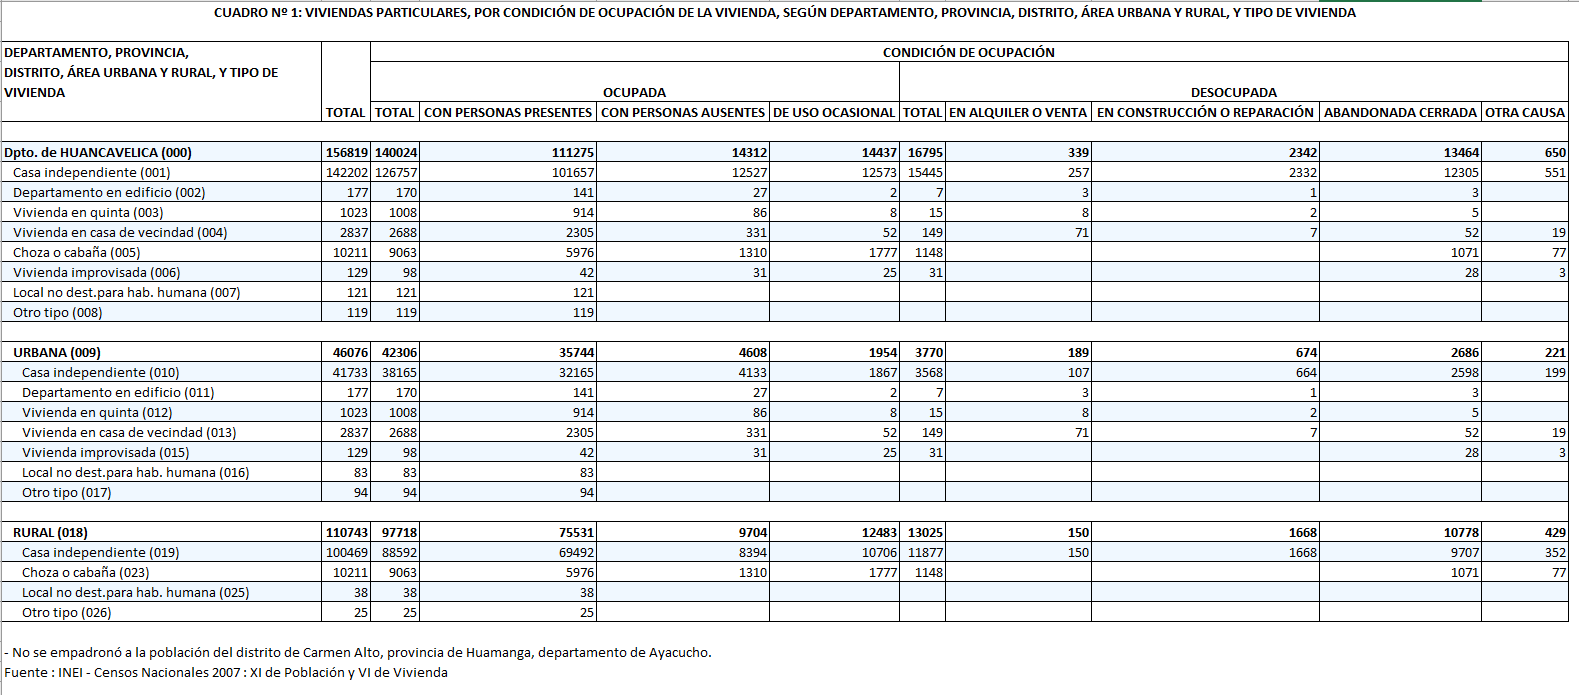
\includegraphics[width=\textwidth]{dataset.png}  % Ajustar el ancho de la imagen
		\caption{Dataset de viviendas en los distritos de Huancavelica.}
		\label{fig:dataset}
	\end{figure}
	
	Para profundizar, se realizó un análisis por distritos en Huancavelica utilizando técnicas de clustering.
	
	\begin{figure}[H]
		\centering
		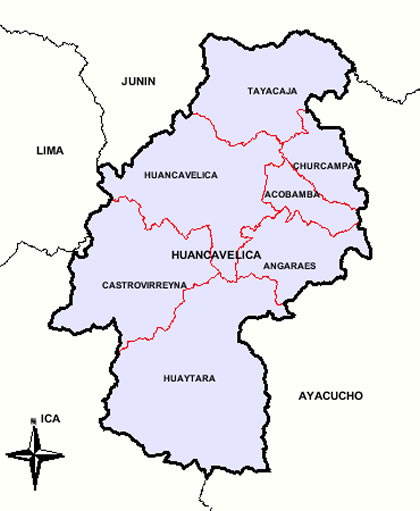
\includegraphics[height=0.4\textheight]{huancavelica.jpg}  % Reduce el tamaño a la mitad de la altura de la página
		\caption{Mapa político de Huancavelica, mostrando sus distritos para análisis de clustering.}
		\label{fig:huancavelica}
	\end{figure}
	
	
	
	\section{Aplicación de K-Means en Huancavelica}
	\subsection{Problema y Objetivo}
	El objetivo de este análisis es realizar una segmentación de los distritos de Huancavelica en tres grupos utilizando el método de clustering K-Means. Las características que se utilizarán para segmentar los distritos son el número de viviendas ocupadas, desocupadas y abandonadas en cada distrito. Esta segmentación nos permitirá clasificar los distritos de acuerdo con su situación socioeconómica relacionada con la ocupación de viviendas.
	
	Planteamos el siguiente escenario:
	\begin{itemize}
		\item Grupo 1 (Alta ocupación): Distritos con alta ocupación de viviendas.
		\item Grupo 2 (Alta desocupación o abandono): Distritos con una gran cantidad de viviendas desocupadas o abandonadas.
		\item Grupo 3 (Mixto): Distritos que tienen una distribución equilibrada de viviendas ocupadas y desocupadas/abandonadas.
	\end{itemize}
	
	\subsection{Datos Utilizados}
	El conjunto de datos utilizado incluye información sobre las viviendas en varios distritos de Huancavelica. Las variables principales son:
	\begin{itemize}
		\item Viviendas Ocupadas: Número de viviendas habitadas.
		\item Viviendas Desocupadas: Viviendas sin habitantes, ya sea en alquiler, en construcción o sin habitar.
		\item Viviendas Abandonadas: Viviendas cerradas o abandonadas por diversas razones.
	\end{itemize}
	
	
	
	\subsection{Proceso de Segmentación utilizando K-Means}
	El algoritmo K-Means se utiliza para clasificar los distritos de acuerdo con sus características. Los pasos son los siguientes:
	
	\begin{enumerate}
		\item \textbf{Normalización de los datos:} Los datos se normalizan para que todas las variables tengan la misma escala y evitar que una variable predomine sobre las demás debido a sus unidades de medida.
		\item \textbf{Aplicación del algoritmo K-Means:} Se aplica el algoritmo K-Means para agrupar los distritos en 3 clústeres. El valor de \( k = 3 \) se elige ya que queremos segmentar los distritos en tres grupos: alta ocupación, alta desocupación o abandono, y mixto.
		\item \textbf{Evaluación y visualización:} El resultado se evalúa utilizando el índice de Silhouette y el índice Davies-Bouldin. También se visualiza la distribución de los distritos en un gráfico.
	\end{enumerate}
	
	\subsection{Resultados}
	El algoritmo K-Means segmentó los distritos de Huancavelica en tres grupos según sus características de viviendas:
	
	\begin{itemize}
		\item Grupo 1 (Alta ocupación): Distritos con un alto número de viviendas ocupadas y un bajo número de viviendas desocupadas.
		\item Grupo 2 (Alta desocupación o abandono): Distritos con una alta cantidad de viviendas desocupadas o abandonadas.
		\item Grupo 3 (Mixto): Distritos con una combinación equilibrada de viviendas ocupadas y desocupadas/abandonadas.
	\end{itemize}
	
	A continuación, se muestra una tabla con la asignación de clústeres para cada distrito.
	
	\begin{table}[h!]
		\centering
		\begin{tabular}{|l|r|r|r|r|}
			\hline
			\textbf{Distrito} & \textbf{Cluster} & \textbf{Descripción del Grupo} \\
			\hline
			Huancavelica       & 0  & Alta ocupación \\
			Acobamba            & 2  & Alta desocupación \\
			Angaraes            & 2  & Alta desocupación \\
			Castrovirreyna      & 1  & Mixto \\
			Churcampa           & 1  & Mixto \\
			Huaytará            & 1  & Mixto \\
			Tayacaja            & 0  & Alta ocupación \\
			\hline
		\end{tabular}
		\caption{Asignación de los distritos de Huancavelica a los grupos según K-Means.}
		\label{tab:clusters}
	\end{table}
	
	\section{Ejemplo en Python}
	A continuación usamos K-Means, presentamos el código en Python que lleva a cabo este análisis:
	
	\begin{lstlisting}[language=Python, caption=Código en Python para aplicar K-Means]
		import pandas as pd
		import numpy as np
		import matplotlib.pyplot as plt
		from sklearn.cluster import KMeans
		from sklearn.preprocessing import StandardScaler
		
		# Crear el dataset basado en la tabla de viviendas en Huancavelica
		data = {
			"Distrito": ["Huancavelica", "Acobamba", "Angaraes", "Castrovirreyna", "Churcampa", "Huaytará", "Tayacaja"],
			"Total_Viviendas": [156819, 12000, 15000, 10000, 11000, 9000, 18000],
			"Viviendas_Ocupadas": [140024, 11000, 13500, 9500, 10500, 8500, 16500],
			"Viviendas_Desocupadas": [16795, 1000, 1500, 500, 500, 500, 1500],
			"Viviendas_Abandonadas": [13464, 700, 1000, 300, 350, 250, 1000]
		}
		
		# Convertir a DataFrame
		df = pd.DataFrame(data)
		
		# Normalizar los datos para evitar sesgos por escala
		scaler = StandardScaler()
		X = scaler.fit_transform(df.iloc[:, 1:])
		
		# Aplicar K-Means
		kmeans = KMeans(n_clusters=3, random_state=42, n_init=10)
		df["Cluster"] = kmeans.fit_predict(X)
		
		# Visualización de los clústeres
		plt.figure(figsize=(10, 6))
		plt.scatter(df["Total_Viviendas"], df["Viviendas_Ocupadas"], c=df["Cluster"], cmap='viridis', s=100, edgecolors='k')
		plt.xlabel("Total de Viviendas")
		plt.ylabel("Viviendas Ocupadas")
		plt.title("Clustering de Distritos de Huancavelica basado en Viviendas")
		plt.colorbar(label="Cluster")
		plt.grid(True)
		plt.show()
		
		# Mostrar resultados en consola
		print(df)
	\end{lstlisting}
	
	Este código utiliza la biblioteca \texttt{scikit-learn} para aplicar K-Means y segmentar los distritos de Huancavelica según sus características de vivienda.
	
	
	\section{Conclusiones}
	La segmentación de los distritos de Huancavelica utilizando el algoritmo K-Means nos permitió clasificar los distritos en tres grupos según sus características de ocupación de viviendas. Esta información es crucial para la toma de decisiones sobre las políticas públicas a implementar en la región, particularmente en lo que respecta a la mejora de la infraestructura y la reducción de la pobreza.
	
	\begin{thebibliography}{15}
		
		\bibitem{fuoc2019} 
		Xavi Font. \textit{Técnicas de Clustering}. FUOC, 2019. 
		Disponible en: \url{https://openaccess.uoc.edu/bitstream/10609/147174/10/AnaliticaDeDatos_Modulo5_TecnicasDeClustering.pdf}
		
		\bibitem{condori2024} 
		Condori Peralta, J. M. \textit{Segmentación de hogares con indicadores socioeconómicos del distrito de Macusani - 2020}. Universidad Nacional del Altiplano, 2024.  
		Disponible en: \url{https://repositorio.unap.edu.pe/bitstream/handle/20.500.14082/21207/Condori_Peralta_Juan_Manuel.pdf?sequence=1&isAllowed=y}
		
		\bibitem{libertadores2021} 
		Álvaro Antonio Forero González. \textit{Análisis de segmentación basado en clustering}. Fundación Universitaria Los Libertadores, 2021.  
		Disponible en: \url{https://repository.libertadores.edu.co/server/api/core/bitstreams/314bcc9e-8b95-46c5-99ec-81f07b466da4/content}
		
		\bibitem{santos2022} 
		Santos, F. L. \textit{Métodos de segmentación de mercados y su aplicación en el análisis de clústeres}. Universidad Tecnológica de Pereira, 2022.  
		Disponible en: \url{https://repositorio.utp.edu.co/handle/11059/13016}
		
		\bibitem{arcos2021} 
		Arcos, A. V. \textit{Clustering y segmentación en mercados: Un análisis comparativo}. Pontificia Universidad Católica del Perú, 2021.  
		Disponible en: \url{https://tesis.pucp.edu.pe/repositorio/handle/20.500.12404/22329}
		
		\bibitem{hernandez2020} 
		Hernández, M. J. \textit{Segmentación y Clustering de clientes en mercados de consumo masivo}. Universidad de Salamanca, 2020.  
		Disponible en: \url{https://gredos.usal.es/handle/10366/146822}
		
		\bibitem{gonzalez2021} 
		González, C. R. \textit{Aplicaciones de técnicas de Clustering en marketing digital}. Universidad de Chile, 2021.  
		Disponible en: \url{https://repositorio.uchile.cl/handle/2250/170011}
		
		\bibitem{garcia2022} 
		García, D. E. \textit{Métodos de Clustering aplicados a grandes bases de datos}. Universidad de Barcelona, 2022.  
		Disponible en: \url{https://www.tdx.cat/handle/10803/286968}
		
		\bibitem{perez2020} 
		Pérez, S. V. \textit{Segmentación de clientes en la industria de retail mediante clustering}. Universidad Autónoma de Madrid, 2020.  
		Disponible en: \url{https://repositorio.uam.es/handle/10486/685685}
		
		\bibitem{rojas2020} 
		Rojas, J. F. \textit{Segmentación de mercados mediante técnicas de clustering y análisis de patrones de consumo}. Universidad de Santiago de Chile, 2020.  
		Disponible en: \url{https://repositorio.usach.cl/handle/123456789/70856}
		
		\bibitem{martinez2019} 
		Martínez, J. D. \textit{Clustering para el análisis de datos masivos en marketing}. Universidad Autónoma de Barcelona, 2019.  
		Disponible en: \url{https://www.tdx.cat/handle/10803/392282}
		
		\bibitem{garcia2023} 
		García, A. L. \textit{Clustering aplicado a la segmentación de usuarios en plataformas digitales}. Universidad de Granada, 2023.  
		Disponible en: \url{https://hera.ugr.es/handle/10481/87998}
		
		\bibitem{rodriguez2021} 
		Rodríguez, F. R. \textit{Segmentación y clustering de consumidores en sectores de alta competencia}. Universidad Nacional Autónoma de México, 2021.  
		Disponible en: \url{https://repositorio.unam.mx/handle/123456789/45522}
		
		\bibitem{diaz2022} 
		Díaz, C. P. \textit{Aplicación de técnicas de clustering para la segmentación de clientes en servicios financieros}. Universidad de Costa Rica, 2022.  
		Disponible en: \url{https://repositorio.ucr.ac.cr/handle/10669/84957}
		
		\bibitem{lopez2021} 
		López, R. S. \textit{Segmentación de consumidores utilizando análisis de clústeres: un enfoque práctico}. Universidad Nacional de San Agustín, 2021.  
		Disponible en: \url{https://repositorio.unsa.edu.pe/handle/20.500.12773/11805}
		
	\end{thebibliography}
	
	
\end{document}
